\documentclass[12pt, a4paper]{report}
\usepackage[utf8]{inputenc}
\usepackage[T1]{fontenc}
\usepackage[utf8]{inputenc}
\usepackage{geometry}
\usepackage{listings}
\usepackage{xcolor}
\usepackage[]{graphicx}
\usepackage[export]{adjustbox}
\usepackage{subcaption}
\makeatletter
\setlength{\@fptop}{0pt}
\makeatother
\usepackage{amsmath} 

\definecolor{codegreen}{rgb}{0.26, 0.61, 0}
\definecolor{codegray}{rgb}{0.5,0.5,5}
\definecolor{codepurple}{rgb}{58,0,0.82}
\definecolor{backcolour}{rgb}{0.80, 0.81, 0.93}

\lstdefinestyle{mystyle}{
    backgroundcolor=\color{backcolour},   
    commentstyle=\color{codegreen},
    keywordstyle=\color{magenta},
    numberstyle=\tiny\color{codegray},
    stringstyle=\color{codepurple},
    basicstyle=\ttfamily\footnotesize,
    breakatwhitespace=false,         
    breaklines=true,                 
    captionpos=b,                    
    keepspaces=true,                 
    numbers=left,                    
    numbersep=5pt,                  
    showspaces=false,                
    showstringspaces=false,
    showtabs=false,                  
    tabsize=2
}

\lstset{style=mystyle}


\title{\textbf{EE2703: Applied Programming Lab\\End Semester
}}


\author{Devaganthan S S\\ EE19B018}
\date{\today}
\begin{document}

\maketitle


\section{Abstract}
This experiment aims to compute and plot the magnetic field $\overrightarrow{B}$ along the z axis from 1cm to 1000cm, and fit the data to the model $B_z= c.z^b$. 

\section{Introduction}
The first step in finding the magnetic field is to compute the vector potential. This can be done with the below equation,
\begin{equation}
    \overrightarrow{A_i_j_k} = \sum_{l=0}^{N-1} \frac{cos(\phi'_l )exp(-jkR_i_j_k_l)\overrightarrow{dl'}}{R_i_j_k_l}
\end{equation}
Where $\overrightarrow{R} = \vec{r} - \overrightarrow{r}'$ and $k = \omega/c = 0.1$ . $\overrightarrow{r}$ is the point where we want the Field, and $\overrightarrow{r'} = a\hat{r'}$ is the point on the loop.

Then we compute the curl of the vector potential to find the magnetic field. Since the assignment requires only the component along the Z-axis, we employ the below equation,
\begin{equation}
    B_z(z) = \frac{A_y(\Delta x,0,z)-A_y(-\Delta x,0,z)-A_x(0,\Delta y,z)+A_x(0,-\Delta y,z)-}{4\Delta x\Delta y}
\end{equation}
We then fit the data to the equation $|B_z| = c.Z^b$ using the least-squares method.
\section{Pseudo Code}
\begin{enumerate}
  \item We break the volume into 3 x 3 x 1000 mesh. This Mesh represents the $\vec{r}_i_j_k$
  \item We break the Loop of wire into 100 sections. The section coordinates are of the form [10cos($\theta$),10sin($\theta$)] where $\theta$ goes from 0 to 2$\pi$ (100 divisions). The direction of current is tangential to the section. So we multiply the coordinates with the direction and plot the quiver plot.
  \item Using the Calc(l) function we generate the terms in the summation (Vector Potential Equation). We add the terms in a ‘for loop’. 
  \item In calc(l),
  \begin{itemize}
      \item We first Compute the $\vec{R_i_j_k}$. This done by subtracting the $\vec{r_i_j_k}$ mesh from $\vec{r_i_j_k}'$. (NumPy Subtraction)
      \item Then Magnitude of $\vec{R_i_j_k}$ is computed and with this the vector potential is computed due to $l^t^h$ section of the for loop.
  \end{itemize}
  \item After computing the Vector Potential, using Equation 2 we can compute the $B_z$. This is done with simple NumPy addition and subtraction of arrays.
  \item To fit the data to the model, we first make the appropriate NumPy Arrays. Then using scipy.linalg we find the necessary parameters.
\end{enumerate}
\section{Implementation and Results}
\subsection{Breaking the volume into a mesh grid (Q2)}
With the function \textbf{meshgrid()}, we create a 3 x 3 x 1000 mesh, with a 1 cm gap between two adjacent mesh points. The below code accomplishes the above tasks.
\noindent
\lstinputlisting[language = python]{code1.py}
\subsection{Plotting the Current Elements in XY plane (Q3)}
The magnitude of the Current is calculated first at each section of the wire. The direction of the current is tangential to the loop. Using matplotlib, the quiver plot is plotted. The below code accomplishes the above task,
\noindent
\lstinputlisting[language = python]{code2.py}
\begin{figure}[h!]
    \centering
    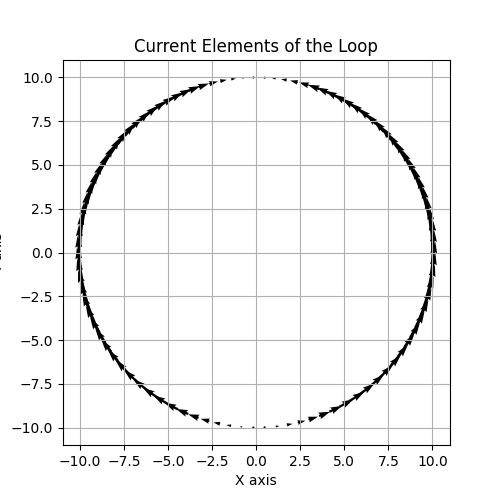
\includegraphics[scale=0.7]{fig1.png} 
    \caption{}
    \label{fig:my_label}
\end{figure}
\subsection{Obtaining the Vectors $\vec{r’_l}$ and $\vec{dl’}$ (Q4)}
 The x and y components of the sections are 10cos($\theta$) and  10sin($\theta$). The $\vec{dl}'$ is the tangential vector to the loop at each section. The below code computes the above vector.
\noindent
\lstinputlisting[language = python]{code3.py}
\subsection{Defining the Function calc(l) and extending it to compute the Vector Potential (Q 5 , Q6) }
Firstly, we compute the $R_i_j_k$ vector and find the magnitude of it at each point on the mesh. Then the function calc(l) computes,
\begin{equation}
    calc(l) = \frac{cos(\phi'_l)exp(-jkR_i_j_k_l)\overrightarrow{dl'}}{R_i_j_k_l}
\end{equation}
Below Code is the Function calc(l),
\noindent
\lstinputlisting[language = python]{code4.py}
\subsection{Computing the Vector Potential (Q7)} 
Using the function calc(l), $A_i_j_k$ is computed in a for loop. Since the number of iterations are 100 and we are adding NumPy arrays, the process is bearable. The trade off is, easier implementation. The below code computes the vector
\noindent
\lstinputlisting[language = python]{code5.py}
\subsection{Computing $\vec{B}$ and Plotting it (Q8 and Q9)}
We compute the Bz component of Magnetic Field using Equation 2.
\noindent
\lstinputlisting[language = python]{code6.py}
\begin{figure}[h!]
    \centering
    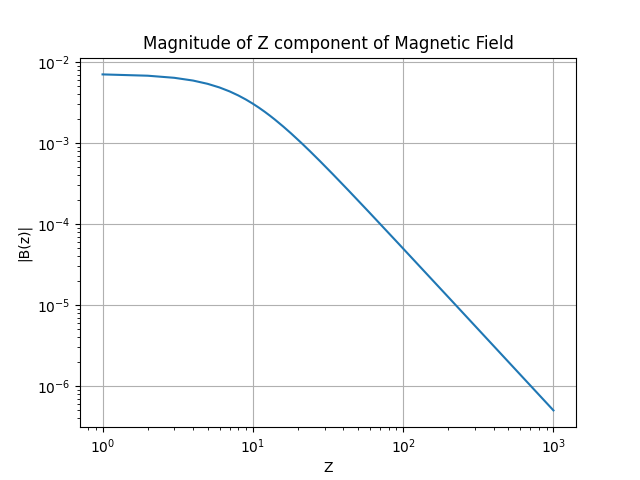
\includegraphics[scale=0.7]{fig2.png} 
    \caption{}
    \label{fig:my_label}
\end{figure}
\vspace{100mm}

\subsection{Fitting the Field to a Model Q10}
Using least squares method, we try fitting the data – $B_z$ into the model , $B_z = cZ^b$.
\begin{equation}
    

\begin{bmatrix}
1 & log(z) \\
\end{bmatrix}\begin{bmatrix}
A\\
B
\end{bmatrix} = \begin{bmatrix}
log(B_z)\\

\end{bmatrix} 
\end{equation}
Here, $c = exp(A)$ and $b =B$
\noindent
\lstinputlisting[language = python]{code4.py}

The Decay Rate Found is -1.9058964119106183. The fitted Plot is,
\begin{figure}[h!]
    \centering
    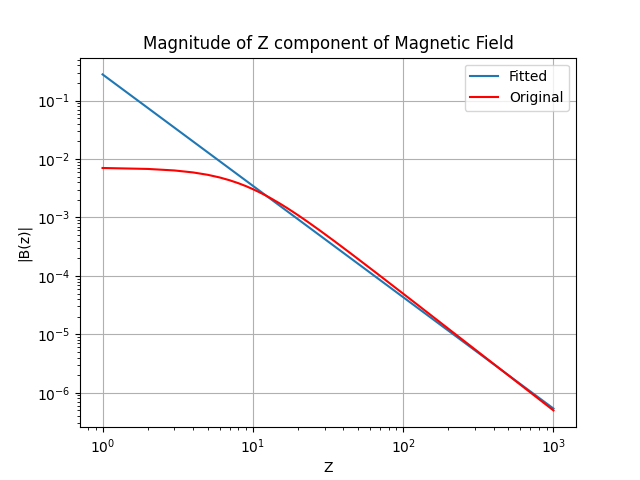
\includegraphics[scale=0.7]{fig3.png} 
    \caption{}
    \label{fig:my_label}
\end{figure}
\vspace{100mm}

\section{Conclusion Q11}
The fitted $B_z$ doesn’t fall of as we expected. We find that the decay value as -1.9058964119106183. Ideally for a static Magnetic field the decay rate is -2. This difference is due to the grid we had chosen. The distance between two mesh points is 1cm, i.e $\Delta X$ = 1cm or $\Delta Y$ = 1cm. The $\Delta X$ we choose, makes a significant effect on B for small values of z. But as z >> x , y the effect is very negligible. Therefore, to get an accurate fit, we have to choose very small $\Delta X$ and $\Delta Y$


\end{document}

